\chapter[Fundamentação]{Fundamentação}
\addcontentsline{toc}{chapter}{Fundamentação}

  \section{Metodologia de desenvolvimento}
  
  A metodologia de desenvolvimento adotada neste projeto é uma adaptação de metodologias gerais de desenvolvimento de
  produtos e serviços. Para a construção deste modelo de desenvolvimento foram selecionadas algumas técnicas de projeto
  de produtos e serviços expostos em algumas obras de Slack (\citeyear{slack99}), Krajewski (\citeyear{krajewski96}) e
  Ramaswamy (\citeyear{ramaswamy96}). Tais trabalhos descrevem formas de estabelecer etapas bem definidas para o desenvolvimento do projeto.
  
  Como estrutura básica do projeto será adotada a seguinte metodologia, dividida em seis etapas:
  
  \begin{figure}[h]
  \begin{center}

  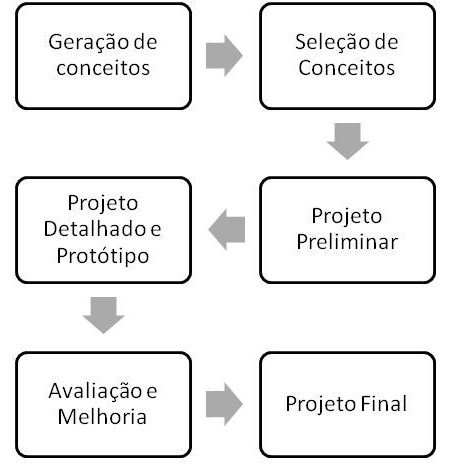
\includegraphics[scale=0.3]{editaveis/figuras/metodologia_de_desenvolvimento}
  \label{Metodologia de desenvolvimento}
  \caption{Metodologia de desenvolvimento}
  \end{center}
  \end{figure}
  \FloatBarrier
  
  A descrição de todas as etapas a cima é relatada a seguir.
  
  \begin{enumerate}
   \parindent=1.25cm
   
   \item Geração de Conceito\\
      
      \noindent
      Divide-se em três:
      
      \noindent
      \subitem \textbf{Geração de ideias}
      
      Foi proposto ao grupo o desenvolvimento de um projeto preliminar de uma planta de abastecimento de água potável a partir 
      da umidade do ar. O projeto a ser realizado deveria ser inovador, de utilidade para seus consumidores finais, viável e
      que utilizasse fontes alternativas de energia para a solução do problema a ser idealizado pelo grupo.
      
      O método utilizado nesta etapa do projeto consiste em produzir reuniões onde todo o grupo estará presente, tais componentes 
      devem fornecer ideias que possam ser debatidas e analisadas por todos, sem descriminação.
      
      \noindent
      \subitem \textbf{Análise de tecnologia}
      
      Nesta fase devem ser realizadas vigorosas pesquisas externas a fim de investigar a existência de tecnologias que realizam o
      trabalho proposto ou que realizam processos similares. 
	    
      A proposta desta etapa é investigar os prós e contras das várias tecnologias pesquisadas e a viabilidade da tecnologia 
      a ser adotada.
      
      \noindent
      \subitem \textbf{Especificação de localização}
      
      Análise de requisitos sobre localização e avaliação das características do problema, a fim de identificar os possíveis 
      consumidores e sua localidade. 
      
      Os potenciais consumidores deste projeto são as famílias nordestinas, que tem suas vidas diariamente sendo ameaçadas 
      devido à falta de reserva de água.
   
  \item Seleção de Conceitos
  
    Esta etapa é responsável por avaliar quais conceitos gerados na fase anterior são relevantes e pela construção do
    embasamento teórico sobre os elementos determinados na etapa anterior. 
  
  \item Projeto Preliminar
  
    Esta etapa busca especificar o serviço e o produto com todos os seus componentes e processos necessários ao funcionamento.
    
    Esta fase é uma das mais importantes de todo o projeto, pois são tomadas decisões que serão o suporte de todo o
    desenvolvimento deste. No projeto preliminar deste projeto foram estabelecidas as seguintes informações principais: 
    
    \begin{itemize}
     \item A região de implementação do projeto será no Município de Acari, situado mais especificamente na região do Seridó, 
	na Mesorregião Central Potiguar, no estado do Rio Grande do Norte, no Brasil.
     
     \item A tecnologia adotada será uma turbina eólica capaz de transformar a umidade do ar em água.
     
     \item Serão adotados critérios quanto a qualidade da água, eficiência da turbina e 
	monitoramento de todo o sistema de captação, armazenamento e distribuição.     
    \end{itemize}
    
  \item Projeto Detalhado e Protótipo
  
    O projeto detalhado se diferencia do projeto preliminar devido às alterações e correções implementadas.
    
    O protótipo do projeto será feito na plataforma de desenho Catia v5\_R19, este processo de construção deve ter como 
    base o projeto detalhado e as dimensões reais do produto, para ser feito em menor escala.

  \item Avaliação e Melhoria
  
    Antes do término do projeto e lançamento do serviço, algumas modificações devem ser feitas em busca de melhorias. 
    Dentre as técnicas utilizadas neste processo, serão recomendadas o Desdobramento da Função Qualidade
    (ou QFD, Quality Function Deployment) e da Análise de Valor.
    
    O Desdobramento da Função Qualidade (QFD) tem como foco principal às necessidades dos clientes, oferecendo as
    alternativas capazes de satisfazê-los. Ou seja, dentro da matriz QFD os requisitos do consumidor (o quê) relacionam-se
    com as características do serviço (como), para que possamos prover mudanças que aumentem a satisfação do cliente.
    
    A Análise de Valor tem como objetivo aumentar o valor relativo de cada componente do serviço prestado, o que pode 
    ser feito através da redução de custos ou através do aumento do nível do serviço. Deve-se, em uma primeira etapa,
    distinguir as funções básicas das secundárias, para em seguida identificar tudo o que possa oferecer diminuição de custos,
    principalmente em funções secundárias; e aumento do valor, em funções básicas.
    
  \item Projeto Final
  
    O projeto final deve conter as alterações propostas por meio das técnicas de avaliação e melhoria, em modelo semelhante
    ao do projeto preliminar, porém de forma extremamente mais completa.
    
  \end{enumerate}

  
  \section{Referencial Teórico}
  
    Esse tópico aborda..
    
    PROCUREM POR TEXTOS DE BASE CIENTÍFICA PARA ESSES TÓPICOS SEGUINTES, E LEMBREM DE REFERENCIAR.
    
    \subsection{Sistema de captação da umidade do ar}
    
    Descrever aqui, o mais detalhado possível, TODAS as tecnologias que pesquisamos.
    
    Descrever, detalhadamente, possíveis materiais que serão utilizados no equipamento.
    
    \subsection{Matriz energética}
    
    Descrever as fontes energéticas pesquisadas e fazer relação com as tecnologias.
    
    Técnicas e métodos de conversão e armazenamento que podem ser utilizados (Descrever cada um).
    
    Descrever como medir a eficiência energética e autonomia do sistema, descrever conceitos o máximo possível.
    
    \subsection{Sistema de monitoramento e controle da qualidade da água}
      
      \subsubsection{Parâmetros de qualidade da água}
      
      Descrever e conceituar parâmetros de qualidade da água
      (Pesquisar na ANA (Agência Nacional de Águas), ADASA (Agência Reguladora de Águas, Energia e Saneamento Básico do DF), CAESB...).
      Pesquisar modelos matemáticos inerentes ao assunto.
    
      \subsubsection{Projeto eletrônico e de controle da planta}
      
      Estudo dos possíveis componentes eletrônicos (descrever detalhadamente) para o monitoramento da qualidade da água.
	Sensores, Microcontroladores, etc..
	
      Descrever métodos de processamento de sinais.
      
      \subsubsection{Interface do sistema de monitoramento da qualidade da água}
      
      Descrever algoritmos que possam ser utilizados.
      
      Pesquisar sistemas de monitoramento de água já existentes e descrevê-los.
      Descrever os dados que precisam ser acompanhados pelo sistema.
      
      Descrever conceitos de IHC (usabilidade, protótipos, etc...).
      
      Pesquisar ferramentas de MockUp e descrevê-las.
    
  \section{Requisitos do sistema}
  
      O projeto possui 4 frentes de requisitos. São elas:
      
      \begin{itemize}
	\item Requisitos do projeto estrutural mecânico do sistema de captação da água e do transporte para a central de armazenamento;
	\item Requisitos do projeto dos circuitos eletrônicos que irão compor o sistema de monitoramento e controle da qualidade da água.
	\item Requisitos do projeto da interface homem-máquina de monitoramento da qualidade da água;
	\item Requisitos do projeto da matriz energética que dará o suporte para o sistema de captação de água e o sistema de monitoramento da qualidade da água;
      \end{itemize}
    
    
    
    